\documentclass[12pt]{article}
\usepackage[margin=1in]{geometry}
\usepackage{alltt}
\usepackage{subfig}
\usepackage{epsfig}
\usepackage{hyperref}
\usepackage{setspace}
\usepackage{gensymb}
\usepackage{libertine} 
\usepackage{siunitx}
\usepackage{amsmath}
\usepackage{placeins}
\usepackage{enumitem}
\newlist{steps}{enumerate}{1}
\setlist[steps, 1]{label = Step \arabic*:}
\usepackage{indentfirst}
\usepackage{float}
\usepackage{lscape}
\usepackage[blocks]{authblk}
\doublespacing
\renewcommand{\baselinestretch}{1}
\setlength{\textheight}{9in}
\setlength{\textwidth}{6.5in}
\setlength{\headheight}{0in}
\setlength{\headsep}{0in}
\setlength{\topmargin}{0in}
\setlength{\oddsidemargin}{0in}
\setlength{\evensidemargin}{0in}
\setlength{\parindent}{.3in}
%%%%%%%%%%%%%%%%%%%%%%%%%%%%%%%%%%%%%%%%%%%%%%%%%%%%%%%%%%%%%%%%%%%%%%
\begin{document}
%%%%%%%%%%%%%%%%%%%%%%%%%%%%%%%%%%%%%%%%%
% LaTeX Template
% Version 1.0 (27/12/12)
%
% This template has been downloaded from:
% http://www.LaTeXTemplates.com
%
% Original author:
% WikiBooks (http://en.wikibooks.org/wiki/LaTeX/Title_Creation)
%
% License:
% CC BY-NC-SA 3.0 (http://creativecommons.org/licenses/by-nc-sa/3.0/)
% 
% Instructions for using this template:
% This title page is capable of being compiled as is. This is not useful for 
% including it in another document. To do this, you have two options: 
%
% 1) Copy/paste everything between \begin{document} and \end{document} 
% starting at \begin{titlepage} and paste this into another LaTeX file where you 
% want your title page.
% OR
% 2) Remove everything outside the \begin{titlepage} and \end{titlepage} and 
% move this file to the same directory as the LaTeX file you wish to add it to. 
% Then add %%%%%%%%%%%%%%%%%%%%%%%%%%%%%%%%%%%%%%%%%
% LaTeX Template
% Version 1.0 (27/12/12)
%
% This template has been downloaded from:
% http://www.LaTeXTemplates.com
%
% Original author:
% WikiBooks (http://en.wikibooks.org/wiki/LaTeX/Title_Creation)
%
% License:
% CC BY-NC-SA 3.0 (http://creativecommons.org/licenses/by-nc-sa/3.0/)
% 
% Instructions for using this template:
% This title page is capable of being compiled as is. This is not useful for 
% including it in another document. To do this, you have two options: 
%
% 1) Copy/paste everything between \begin{document} and \end{document} 
% starting at \begin{titlepage} and paste this into another LaTeX file where you 
% want your title page.
% OR
% 2) Remove everything outside the \begin{titlepage} and \end{titlepage} and 
% move this file to the same directory as the LaTeX file you wish to add it to. 
% Then add %%%%%%%%%%%%%%%%%%%%%%%%%%%%%%%%%%%%%%%%%
% LaTeX Template
% Version 1.0 (27/12/12)
%
% This template has been downloaded from:
% http://www.LaTeXTemplates.com
%
% Original author:
% WikiBooks (http://en.wikibooks.org/wiki/LaTeX/Title_Creation)
%
% License:
% CC BY-NC-SA 3.0 (http://creativecommons.org/licenses/by-nc-sa/3.0/)
% 
% Instructions for using this template:
% This title page is capable of being compiled as is. This is not useful for 
% including it in another document. To do this, you have two options: 
%
% 1) Copy/paste everything between \begin{document} and \end{document} 
% starting at \begin{titlepage} and paste this into another LaTeX file where you 
% want your title page.
% OR
% 2) Remove everything outside the \begin{titlepage} and \end{titlepage} and 
% move this file to the same directory as the LaTeX file you wish to add it to. 
% Then add \input{./title_page_1.tex} to your LaTeX file where you want your
% title page.
%
%%%%%%%%%%%%%%%%%%%%%%%%%%%%%%%%%%%%%%%%%

%----------------------------------------------------------------------------------------
%	PACKAGES AND OTHER DOCUMENT CONFIGURATIONS
%----------------------------------------------------------------------------------------

%\documentclass[12pt]{article}

%\begin{document}

\begin{titlepage}

\newcommand{\HRule}{\rule{\linewidth}{0.5mm}} % Defines a new command for the horizontal lines, change thickness here

\center % Center everything on the page
 
%----------------------------------------------------------------------------------------
%	HEADING SECTIONS
%----------------------------------------------------------------------------------------

%\textsc{\LARGE }\\[1.2cm] % Name 
%\textsc{\Large }\\[0.5cm] % Major heading
%\textsc{\large }\\[0.5cm] % Minor heading \\


%----------------------------------------------------------------------------------------
%	TITLE SECTION
%----------------------------------------------------------------------------------------

\HRule \\[0.4cm]
{ \huge \bfseries Numerical Approximation of a Derivative Using the Method of Central Difference}\\[0.4cm] % Title of your document
\HRule \\[1.5cm]

\textsc{\bf {\large November 16, 2018}} \\
	   %{\bf {\large Performed on November 1, 2018}} \\
	   \vspace{0.8in}
	   
%----------------------------------------------------------------------------------------
%	AUTHOR SECTION
%----------------------------------------------------------------------------------------

%\begin{minipage}{0.4\textwidth}
%\begin{flushleft} \large
\emph{Author:}\\
Jonathan Duarte \\ % Your name
%Email: 
%\end{flushleft}
%\end{minipage}
~
%\begin{minipage}{0.4\textwidth}
%\begin{flushright} \large
%\emph{Assistant} \\
% \\ % Supervisor's Name
%Email: sample1.edu
%\end{flushright}
%\end{minipage}\\[4cm]

% If you don't want a supervisor, uncomment the two lines below and remove the section above
%\Large \emph{Author:}\\
%John \textsc{Smith}\\[3cm] % Your name

%----------------------------------------------------------------------------------------
%	DATE SECTION
%----------------------------------------------------------------------------------------

%{\large \today}\\[2cm] % Date, change the \today to a set date if you want to be precise

%----------------------------------------------------------------------------------------
%	LOGO SECTION
%----------------------------------------------------------------------------------------

%\includegraphics[width=3.0in]{} % Include a department/university logo - this will require the graphicx package
 
%----------------------------------------------------------------------------------------

\vfill % Fill the rest of the page with whitespace

\end{titlepage} to your LaTeX file where you want your
% title page.
%
%%%%%%%%%%%%%%%%%%%%%%%%%%%%%%%%%%%%%%%%%

%----------------------------------------------------------------------------------------
%	PACKAGES AND OTHER DOCUMENT CONFIGURATIONS
%----------------------------------------------------------------------------------------

%\documentclass[12pt]{article}

%\begin{document}

\begin{titlepage}

\newcommand{\HRule}{\rule{\linewidth}{0.5mm}} % Defines a new command for the horizontal lines, change thickness here

\center % Center everything on the page
 
%----------------------------------------------------------------------------------------
%	HEADING SECTIONS
%----------------------------------------------------------------------------------------

%\textsc{\LARGE }\\[1.2cm] % Name 
%\textsc{\Large }\\[0.5cm] % Major heading
%\textsc{\large }\\[0.5cm] % Minor heading \\


%----------------------------------------------------------------------------------------
%	TITLE SECTION
%----------------------------------------------------------------------------------------

\HRule \\[0.4cm]
{ \huge \bfseries Numerical Approximation of a Derivative Using the Method of Central Difference}\\[0.4cm] % Title of your document
\HRule \\[1.5cm]

\textsc{\bf {\large November 16, 2018}} \\
	   %{\bf {\large Performed on November 1, 2018}} \\
	   \vspace{0.8in}
	   
%----------------------------------------------------------------------------------------
%	AUTHOR SECTION
%----------------------------------------------------------------------------------------

%\begin{minipage}{0.4\textwidth}
%\begin{flushleft} \large
\emph{Author:}\\
Jonathan Duarte \\ % Your name
%Email: 
%\end{flushleft}
%\end{minipage}
~
%\begin{minipage}{0.4\textwidth}
%\begin{flushright} \large
%\emph{Assistant} \\
% \\ % Supervisor's Name
%Email: sample1.edu
%\end{flushright}
%\end{minipage}\\[4cm]

% If you don't want a supervisor, uncomment the two lines below and remove the section above
%\Large \emph{Author:}\\
%John \textsc{Smith}\\[3cm] % Your name

%----------------------------------------------------------------------------------------
%	DATE SECTION
%----------------------------------------------------------------------------------------

%{\large \today}\\[2cm] % Date, change the \today to a set date if you want to be precise

%----------------------------------------------------------------------------------------
%	LOGO SECTION
%----------------------------------------------------------------------------------------

%\includegraphics[width=3.0in]{} % Include a department/university logo - this will require the graphicx package
 
%----------------------------------------------------------------------------------------

\vfill % Fill the rest of the page with whitespace

\end{titlepage} to your LaTeX file where you want your
% title page.
%
%%%%%%%%%%%%%%%%%%%%%%%%%%%%%%%%%%%%%%%%%

%----------------------------------------------------------------------------------------
%	PACKAGES AND OTHER DOCUMENT CONFIGURATIONS
%----------------------------------------------------------------------------------------

%\documentclass[12pt]{article}

%\begin{document}

\begin{titlepage}

\newcommand{\HRule}{\rule{\linewidth}{0.5mm}} % Defines a new command for the horizontal lines, change thickness here

\center % Center everything on the page
 
%----------------------------------------------------------------------------------------
%	HEADING SECTIONS
%----------------------------------------------------------------------------------------

%\textsc{\LARGE }\\[1.2cm] % Name 
%\textsc{\Large }\\[0.5cm] % Major heading
%\textsc{\large }\\[0.5cm] % Minor heading \\


%----------------------------------------------------------------------------------------
%	TITLE SECTION
%----------------------------------------------------------------------------------------

\HRule \\[0.4cm]
{ \huge \bfseries Numerical Approximation of a Derivative Using the Method of Central Difference}\\[0.4cm] % Title of your document
\HRule \\[1.5cm]

\textsc{\bf {\large November 16, 2018}} \\
	   %{\bf {\large Performed on November 1, 2018}} \\
	   \vspace{0.8in}
	   
%----------------------------------------------------------------------------------------
%	AUTHOR SECTION
%----------------------------------------------------------------------------------------

%\begin{minipage}{0.4\textwidth}
%\begin{flushleft} \large
\emph{Author:}\\
Jonathan Duarte \\ % Your name
%Email: 
%\end{flushleft}
%\end{minipage}
~
%\begin{minipage}{0.4\textwidth}
%\begin{flushright} \large
%\emph{Assistant} \\
% \\ % Supervisor's Name
%Email: sample1.edu
%\end{flushright}
%\end{minipage}\\[4cm]

% If you don't want a supervisor, uncomment the two lines below and remove the section above
%\Large \emph{Author:}\\
%John \textsc{Smith}\\[3cm] % Your name

%----------------------------------------------------------------------------------------
%	DATE SECTION
%----------------------------------------------------------------------------------------

%{\large \today}\\[2cm] % Date, change the \today to a set date if you want to be precise

%----------------------------------------------------------------------------------------
%	LOGO SECTION
%----------------------------------------------------------------------------------------

%\includegraphics[width=3.0in]{} % Include a department/university logo - this will require the graphicx package
 
%----------------------------------------------------------------------------------------

\vfill % Fill the rest of the page with whitespace

\end{titlepage}
\newpage
%%%%%%%%%%%%%%%%%%%%%%%%%%%%%%%%%%%%%%%%%%%%%%%%%%%%%%%%%%%%%%%%%%%%%%%%%%%%%%%%%%%%%%%%%%%%%%
\section*{Abstract}
\begin{doublespace}
The purpose of this \textbf{FORTRAN} program was to perform a numerical approximation of a derivative using the central difference method. A smooth function $y$ = $\sin$($10x$), where $x\in[-1,1]$, was used to obtain the end result of the estimate as well as its numerical stability. In order to obtain the central difference of a smooth function, a Taylor Series expansion was taken around some neighborhood of a point $x$. After obtaining a finite approximation, it was possible to estimate the derivative at $x$ = $x_{i}$ by using values from the left side of $y$ as well as to the right. Since the end points are not valid around the neighborhood of $x$, a special one-sided formul\ae was constructed. It can be shown that at $N$ = 6, the special one-sided formul\ae can be written in matrix form, namely {\bf D}. With {\bf y} being the independent variable of the function and {\bf D} being a matrix, it was possible to estimate the derivatives {\bf $y'$} by a matrix-vector multiplication. The end result illustrates that by taking the second derivative of $y$, the function's discrete points collapsed more accurately than the first derivative. An error analysis was then conducted for $y'$ = $10\cos(10x)$ at $y'(0)$ = 10 using a log-log plot which resulted in the decrease in truncation error as the magnitude increased. 
\end{doublespace}

\newpage
%%%%%%%%%%%%%%%%%%%%%%%%%%%%%%%%%%%%%%%%%%%%%%%%%%%%%%%%%%%%%%%%%%%%%%%%%%%%%%%%%%%%%%%%%%
\section*{Numerical Analysis}
\begin{doublespace}
As described in the {\bf Abstract}, a smooth function was used for the method of central difference, namely 
\end{doublespace}

\begin{eqnarray}
y = \sin(10x), \quad x \in [-1,1] \label{ee1}
\end{eqnarray}

\begin{doublespace}
\noindent
In order to arrive at that conclusion it is necessary to derive the central difference method. In a general smooth function, the central difference method is first obtained by a Taylor Series expansion taken around some neighborhood of a point $x$. The neighboring $x$ values that surround the point are:
\end{doublespace}

\begin{eqnarray*}
...,x-3h,x-2h,x-h,x,x+h,x+2h,x+3h,...
\end {eqnarray*}

\begin{doublespace}
\noindent
Using Taylor's theorem, we have:
\end{doublespace}

\begin{eqnarray*}
y(x+h)=y(x)+y'(x)h+{\frac{1}{2}}y''(\lambda_{2})h^{2}
\end{eqnarray*}

\begin{doublespace}
\noindent
By canceling out the higher order terms and reworking the equation, we have:
\end{doublespace}

\begin{eqnarray*}
y'(x) \approx \dfrac{y(x+h)-y(x)}{h}
\end{eqnarray*}

\begin{doublespace}
\noindent
which is the forward difference approximation. If $x$ is the central point of the approximation, it can be shown that:
\end{doublespace}

\begin{eqnarray*}
y'(x) \approx \dfrac{y(x+h)-y(x-h)}{2h}
\end{eqnarray*}

\begin{doublespace}
\noindent
is the central difference formula approximation. To simplify the previous approximation, let's suppose we want a precise estimate such that $x+h$ is the iteration of $y_{i+1}$, $x-h$ is the iteration of $y_{i-1}$ and $y'(x)$ = $y'_{i}$. Lets also suppose that, $h$ = $\Delta{x}$ where $\Delta{x}$ = $\frac{b-a}{N}$, $x\in[a,b]$, and $N$ is the number of spaces uniformly distributed around point $x$ = $x_{i}$. Our new approximation becomes:
\end{doublespace}

\begin{eqnarray*}
y'_{i} \approx \dfrac{y_{i+1}-y{i-1}}{2\Delta{x}}, \quad i = 2,...,N
\end{eqnarray*}

\begin{doublespace}
\noindent
The estimate $y'_{i}$ does not become valid when the end points, $y'_{i}$ and $y'_{N+1}$, because there are no values for $y_{0}$ or $y_{N+2}$. Thus a special one-sided formul\ae was constructed for the end points, namely:
\end{doublespace}

\begin{eqnarray}
y'_{1} = \dfrac{-3y_{1}+4y_{2}-y_{3}}{2\Delta{x}}, \label{ee2}
\end{eqnarray}
\begin{eqnarray}
y'_{N+1} = \dfrac{y_{N-1}-4y_{N}+3y_{N+1}}{2\Delta{x}} \label{ee3}
\end{eqnarray}

\noindent
All of the $y'_{i}$ can be written in matrix form with $N$ = 6. To illustrate we now have:

$$\underbrace{
\left[ \begin{array}{c} 
	y'_{1} \\ 
	y'_{2} \\ 
	y'_{3} \\
	y'_{4} \\
	y'_{5} \\
	y'_{6} \\
	y'_{7} 
\end{array} \right]}_{\textbf y'} = 
\underbrace{
\begin{bmatrix} 
	-\frac{3}{2\Delta{x}} & \frac{4}{2\Delta{x}} & -\frac{1}{2\Delta{x}} & 0 & 0 & 0 & 0 \\
	-\frac{1}{2\Delta{x}} & 0 & \frac{1}{2\Delta{x}} & 0 & 0 & 0 & 0 \\
	0 & -\frac{1}{2\Delta{x}} & 0 & \frac{1}{2\Delta{x}} & 0 & 0 & 0 \\
	0 & 0 & -\frac{1}{2\Delta{x}} & 0 & \frac{1}{2\Delta{x}} & 0 & 0 \\
	0 & 0 & 0 & -\frac{1}{2\Delta{x}} & 0 & \frac{1}{2\Delta{x}} & 0 \\
	0 & 0 & 0 & 0 & -\frac{1}{2\Delta{x}} & 0 & \frac{1}{2\Delta{x}} \\
	0 & 0 & 0 & 0 & \frac{1}{2\Delta{x}} & -\frac{4}{2\Delta{x}} & \frac{3}{2\Delta{x}}
\end{bmatrix}}_{\textbf D}
\underbrace{
\left[ \begin{array}{c} 
	y_{1} \\ 
	y_{2} \\ 
	y_{3} \\ 
	y_{4} \\ 
	y_{5} \\ 
	y_{6} \\ 
	y_{7}
\end{array} \right]}_{\textbf y}$$
\\
\begin{doublespace}
\noindent
This is of the form:
\end{doublespace}

\begin{eqnarray}
{\textbf y'} = {\textbf D} \cdot {\textbf y} \label{ee4}
\end{eqnarray}
\\ 
\begin{doublespace}
\noindent
{\textbf D} can be reduced into:
\end{doublespace}

\begin{equation*}
{\textbf D} = \frac{1}{2\Delta{x}}
\begin{bmatrix} 
	-3 & 4 & -1 & 0 & 0 & 0 & 0 \\
	-1 & 0 & 1 & 0 & 0 & 0 & 0 \\
	0 & -1 & 0 & 1 & 0 & 0 & 0 \\
	0 & 0 & -1 & 0 & 1 & 0 & 0 \\
	0 & 0 & 0 & -1 & 0 & 1 & 0 \\
	0 & 0 & 0 & 0 & -1 & 0 & 1 \\
	0 & 0 & 0 & 0 & 1 & -4 & 3
\end{bmatrix}, \quad (N=6)
\end{equation*}
\\
\begin{doublespace}
\noindent
In index notation, equation (\ref{ee4}) can be written as:
\end{doublespace}

\begin{eqnarray}
y'_{i} = \sum_{j=1}^{N+1} D_{{i}{j}}y_{j}
\end{eqnarray}

\begin{doublespace}
\noindent
Higher order derivatives can also be estimated by a simple repeated application of derivative matrix {\textbf D}, which leads equation (\ref{ee4}) to become:
\end{doublespace}

\begin{eqnarray}
{\textbf y''} = {\textbf D} \cdot {\textbf D} \cdot {\textbf y} \label{ee5}
\end{eqnarray}

\begin{doublespace}
\noindent
Similarly to before, the index notation of the second derivative in equation (\ref{ee5}) is as follows:
\end{doublespace}

\begin{eqnarray}
y''_{i} = \sum_{j=1}^{N+1} D_{{i}{j}} \sum_{k=1}^{N+1} D_{{j}{k}}y_{k} = \sum_{j=1}^{N+1} \sum_{k=1}^{N+1} D_{{i}{j}} D_{{j}{k}}y_{k} \label{ee6}
\end{eqnarray}

\begin{doublespace}
In order to develop a complete solution for the central difference program in {\bf Appendix A}, it is imperative to allocate any sized dimensional array when doing large iterative calculations. This is done so that the values of the element of a dimensional array can have a shape to store the solution and iterate them in a manner that is specified by the user. Afterwards, integers and counters are initialized to help iterate the loop. In this program, we are working with a square matrix and a single vector. Therefore, initializing the dimensions for matrix-vector multiplication will insure that the proper element of a dimensional array are used and stored iteratively. In a nested do loop the matrix-vector multiplication technique was first applied to estimate the first and second derivatives of equation \ref{ee1} at each $x_{i}$. Then the \textbf{FORTRAN} intrinsic \textbf{matmul} feature was used to obtain the same result as in the nested loop. If a user inputs $N$ = 6 as the number of $N$+1 uniformly distributed points, then the program estimates the first and second derivatives at $x_{i}$, super-posed with each respective solution. Evidently, the discrete points in Figure (1a) demonstrate discrepancies along the curve of the first derivative. However, in Figure (1b), the plot seem to collapsed accurately into the curve, confirming the method of central difference. An error analysis also was conducted for the first derivative of $y'$ = $10\cos(10x)$ at $y'(0)$ = 10 as seen in Figure (2). At $x_{i}$=0 of this log-log plot, the magnitude of the error varied as a function of $\Delta{x}$. It is also evident that the error of $\Delta{x}$ decreases as the order of magnitude $N$ increases. However, only four plots demonstrate this result. One hypothesis is the use single precision. If double precision numbers were used, an $10^{4}$ may appear on the graph.
\end{doublespace}

\newpage

%%%%%%%%%%%%%%%%%%%%%%%%%%%%%%%%%%%%%%%%%%%%%%%%%%%%%%%%%%%%%%%%%%%%%%%%%%%%%%
\begin{landscape}
\begin{figure}[ht]
\begin{center}
\subfloat[]{
\label{fig:subfig:a}
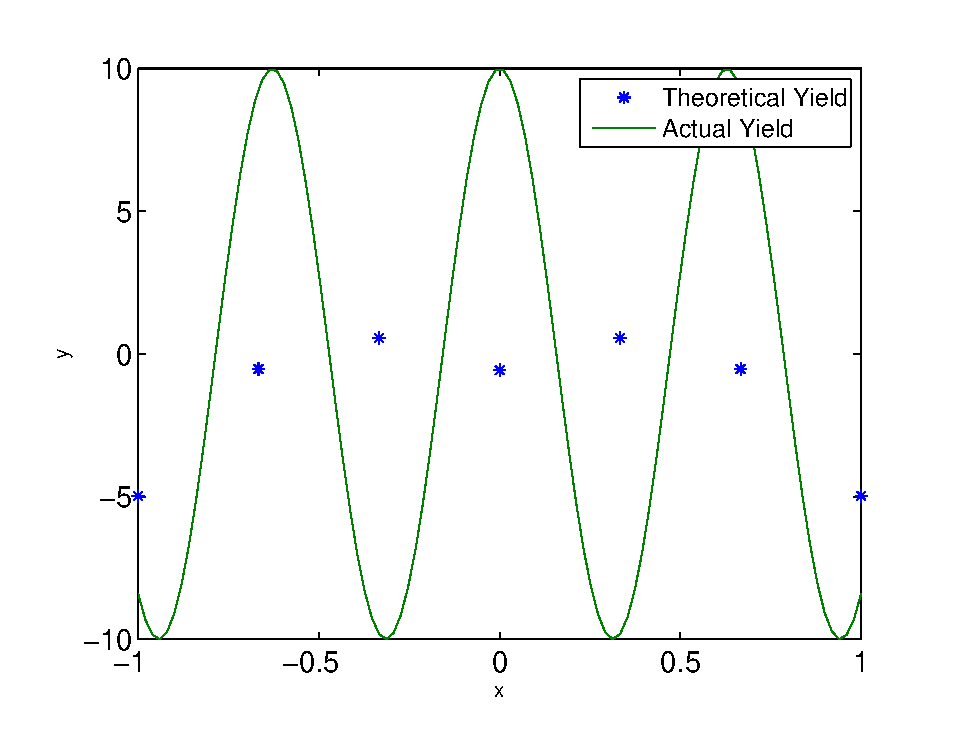
\includegraphics[width=3.2in]{graph1.eps}}
\subfloat[]{
\label{fig:subfig:b}
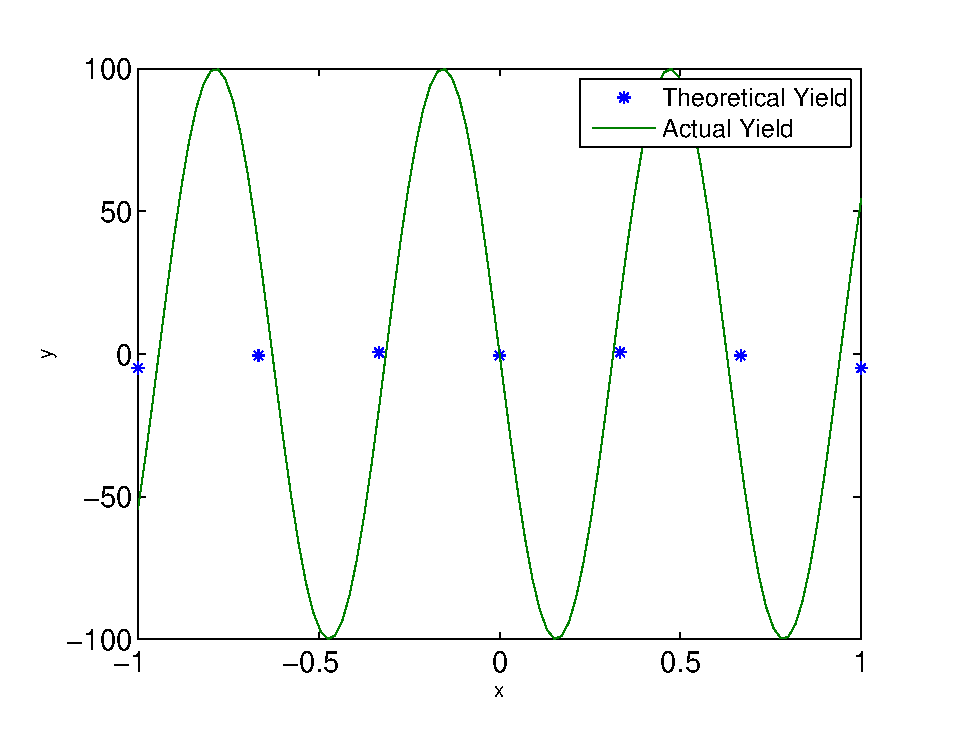
\includegraphics[width=3.2in]{graph2.eps}}
\end{center}
\caption{Representation of a sinusoidal matrix-vector multiplication on the first derivative (a) and second derivative (b) based on equation \ref{ee1} while $x \in$ [-1,1]}
\label{fig:subfig}
\end{figure}
\end{landscape}
%%%%%%%%%%%%%%%%%%%%%%%%%%%%%%%%%%%%%%%%%%%%%%%%%%%%%%%%%%%%%%%%%%%%%%%%%%%%%%
\begin{landscape}
\begin{figure}[ht]
\begin{center}
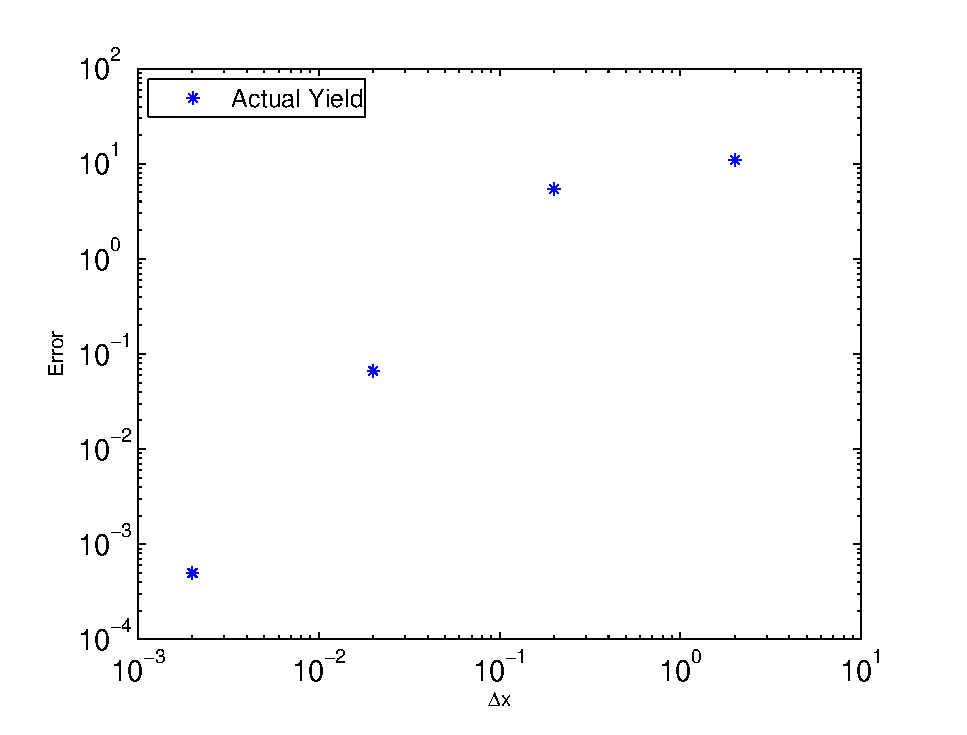
\includegraphics[width=3.2in]{graph3.eps}
\caption{A log-log demonstration displaying the proximity of equation $y'$ = $10\cos(10x)$ as the value of N spans several orders in magnitude}
\label{fig3}
\end{center}
\end{figure}
\end{landscape}

\newpage
%%%%%%%%%%%%%%%%%%%%%%%%%%%%%%%%%%%%%%%%%%%%%%%%%%%%%%%%%%%%%%%%%%%%%%%%%%%%%%
\section*{Appendix A: FORTRAN Code}
\begingroup
\fontsize{8pt}{10pt}\selectfont
\begin{verbatim}
program matrix  ! program to approximate y(x); Read from LEFT TO RIGHT
implicit none   ! [!!!] indicates matmul [!!!!!] indicates do loops
integer :: n, istop, q
integer (kind=4) :: i,j,f
real (kind=4), dimension(:,:), allocatable :: D
real (kind=4), dimension(:), allocatable :: gp, gdp, g, gpb, gpc
real (kind=4):: x, dx, y, k, error
open(unit=20,file='matrix.out')
print*,' Input ONE desired integer for N amount of spaces'  
read*,n
dx = 2./n
k=1./(2*dx)
print*, 'k= ',k            
allocate(gpc(1:n+1))         
allocate(gpb(1:n+1))                 
allocate(gp(1:n+1))         
allocate(gdp(1:n+1))        
allocate(g(1:n+1))           
allocate(D(1:n+1,1:n+1))     
D(1,1) = -3*k 
D(1,2) = 4*k  
D(1,3) = -1*k
D(n+1,n-1) = 1*k
D(n+1,n) = -4*k
D(n+1,n+1) = 3*k
do i=2,n !!!!!
D(i,i-1) = -1*k
D(i,i+1) = 1*k
enddo
print*,'Discrete [Matrix]'
print*, D
istop = n+1
i=1
q=1
do while(i<=istop) !!!!!
	x=-1+(2./n)*(i-1)
	y=sin(10.*x)
	G(q) = y
	i=i+1
	q=q+1
enddo
print*, 'F of (x) [Vector]'
print*, G
do i=1, istop [!!!!!]
   do q=1, istop
   gpb(i)=gpb(i)+D(i,q)*G(q)
   enddo
enddo
do i=1, istop [!!!!!]
   do q=1, istop
   gpc(i)=gpc(i)+D(i,q)*gpb(q)
   enddo
enddo
gp=matmul(D,G) [!!!]
gdp=matmul(D,gp) [!!!]
print*, 'First D Nested LOOP [!!!!!]'
print*,gpb
print*, 'First D MATMUL [!!!]'
print*,gp
print*, 'Second D Nested [!!!!!]'
print*,gpc
print*, 'Second D MATMUL [!!!]'
print*,gdp
print*,'error',10.-gpb((n/2.)+1.)
end program matrix             
\end{verbatim}
\endgroup
%%%%%%%%%%%%%%%%%%%%%%%%%%%%%%%%%%%%%%%%%%%%%%%%%%%%%%%%%%%%%%%%%%%%%%%%%%%%%%
\end{document}
